% Straight up stealing preamble from Eli Holmes 
%%%%%%%%%%%%%%%%%%%%%%%%%%%%%%%%%%%%%%START PREAMBLE THAT IS THE SAME FOR ALL EXAMPLES
\documentclass{article}

%Required: You must have these
\usepackage{Sweave}
\usepackage{graphicx}
\usepackage{tabularx}
\usepackage{hyperref}
\usepackage{natbib}
\usepackage{pdflscape}
\usepackage{array}
\usepackage{gensymb}
%\usepackage{authblk}
\renewcommand{\baselinestretch}{1.8}
%\usepackage{lineno}
%\usepackage[backend=bibtex]{biblatex}
%Strongly recommended
 %put your figures in one place
 
%you'll want these for pretty captioning
\usepackage[small]{caption}

\setkeys{Gin}{width=0.8\textwidth} %make the figs 50 perc textwidth
\setlength{\captionmargin}{30pt}
\setlength{\abovecaptionskip}{0pt}
\setlength{\belowcaptionskip}{10pt}
% manual for caption http://www.dd.chalmers.se/latex/Docs/PDF/caption.pdf

%Optional: I like to muck with my margins and spacing in ways that LaTeX frowns on
%Here's how to do that
 \topmargin -2cm 
 \oddsidemargin -0.04cm 
 \evensidemargin -0.04cm % same as oddsidemargin but for left-hand pages
 \textwidth 16.59cm
 \textheight 22.94cm 
 %\pagestyle{empty} % Uncomment if don't want page numbers
 \parskip 7.2pt  % sets spacing between paragraphs
 %\renewcommand{\baselinestretch}{1.5} 	% Uncomment for 1.5 spacing between lines
\parindent 0pt% sets leading space for paragraphs
\usepackage{setspace}
%\doublespacing

%Optional: I like fancy headers
\usepackage{fancyhdr}
\pagestyle{fancy}
\fancyhead[LO]{Experimental climate change}
\fancyhead[RO]{2018}

%%%%%%%%%%%%%%%%%%%%%%%%%%%%%%%%%%%%%%END PREAMBLE THAT IS THE SAME FOR ALL EXAMPLES

%Start of the document
\begin{document}

% \SweaveOpts{concordance=TRUE}
\bibliographystyle{/Users/aileneettinger/citations/Bibtex/styles/ecol_let.bst}

\title{How does soil moisture interact with temperature to affect phenology?}
\author[1,2,a]{A.K. Ettinger}

%\author[3,b]{I. Chuine}

%\author[4,5,c]{B.I. Cook}

%\author[6,d]{J.S. Dukes}

%\author[7,e]{A.M. Ellison}

%\author[8,f]{M.R. Johnston}

%\author[9,g]{A.M. Panetta}

%\author[10,h]{C.R. Rollinson}

%\author[11,12,i]{Y. Vitasse}

\author[1,8,13,j]{E.M. Wolkovich}

%\affil[1]{Arnold Arboretum of Harvard University, Boston, Massachusetts 02131, USA}

%\affil[2]{Tufts University, Medford, Massachusetts 02155, USA}

%\affil[3]{CEFE UMR 5175, CNRS, Universit\'e de Montpellier,Universit\'e Paul-Val\'ery Montpellier, EPHE IRD, Montpellier, France}

%\affil[4]{Lamont-Doherty Earth Observatory, Columbia University, Palisades, New York 10964, USA}

%\affil[5]{NASA Goddard Institute for Space Studies, New York, New York 10025, USA}

%\affil[6]{Department of Forestry and Natural Resources
%and Department of Biological Sciences, Purdue University, West Lafayette, Indiana 47907, USA}

%\affil[7]{Harvard Forest, Harvard University, Petersham, Massachusetts 01366, USA}

%\affil[8]{Department of Organismic and Evolutionary Biology, Harvard University, Cambridge, Massachusetts 02138, USA}

%\affil[9]{Department of Ecology and Evolutionary Biology, University of Colorado, Boulder, Colorado 80309, USA}

%\affil[10]{The Morton Arboretum, Lisle, Illinois 60532, USA}

%\affil[11]{Institute of Geography, University of Neuch\^atel, Neuch\^atel, Switzerland}

%\affil[12]{Swiss Federal Institute for Forest, Snow and Landscape Research WSL, Neuch\^atel, Switzerland}

%\affil[13]{Forest \& Conservation Sciences, Faculty of Forestry, University of British Columbia, Vancouver, BC, Canada}

%\affil[a]{Corresponding author; email: aettinger@fas.harvard.edu; phone: 781-296-4821; mailing address: 1300 Centre Street, Boston, Massachusetts 02140, USA }

%\affil[b]{isabelle.chuine@cefe.cnrs.fr}

%\affil[c]{bc9z@ldeo.columbia.edu}

%\affil[d]{jsdukes@purdue.edu}

%\affil[e]{aellison@fas.harvard.edu}

%\affil[f]{mjohnston@g.harvard.edu}

%\affil[g]{anne.panetta@colorado.edu}

%\affil[h]{crollinson@mortonarb.org}

%\affil[i]{yann.vitasse@wsl.ch}

%\affil[j]{e.wolkovich@ubc.ca}


\date{\today}
\maketitle %put the fancy title on
%\tableofcontents %add a table of contents

%\textbf{Statement of authorship} %Statement of authorship: Contributions by authors should be listed on the title page and will be printed at the end of the manuscript. This statement should be appropriate to the study described in the manuscript and should clarify who designed the study, who performed the research, who provided new methods or materials, and who wrote the manuscript. We encourage concise statements such as ?JW performed phylogenetic analyses, MH collected data, performed modeling work and analyzed output data, and PK performed the meta-analysis. MH wrote the first draft of the manuscript, and all authors contributed substantially to revisions.?
%All authors conceived of this manuscript, which was inspired by our discussions at a Radcliffe Exploratory Seminar in 2016, and all authors contributed to manuscript revisions. AKE and EMW conceived of the idea for the literature review, database compilation, and related Radcliffe Exploratory Seminar. AKE compiled the datasets; AKE analyzed the data and created the figures; AKE wrote the manuscript.

%\textbf{Data Accessibility} %Data accessibility statement: The statement must confirm that, should the manuscript be accepted, the data supporting the results will be archived in an appropriate public repository such as Dryad or Figshare and the data DOI will be included at the end of the article.
%The MC3E database will be available at KNB \citep{ettinger2018}, along with all R code from the analyses included in this paper. (Currently, metadata are published there; the full database and R code are available to reviewers on github.) 

%\textbf{Running title} 
%\textbf{Key words} global warming, warming experiment, microclimate, soil moisture, phenology, budburst, direct and indirect effects, active-warming, target temperature


\clearpage
%%%%%%%%%%%%%%%%%%%%%%%%%%%%%%%%%%%%%%%%%%%%%%%%%%%
%\linenumbers

\section*{Question/goals}
\begin{enumerate}
\item{How does soil moisture affect phenology?}
\item{Does the effect of soil moisture on phenology differ between experiments and observational data?}
\end{enumerate}
\section*{Approach}
\begin{enumerate}
\item{Compile phenology data that goes with climate data in MC3E database. (Name this database!)}
\item{Fit models with soil moisture, temperature, and interaction to phenology data (budburst, leafout, flowering, fruiting, senesence? (See what phenophases have enough data.)}
\item{Compile Duke and Harvard Forest phenology and climate data.}
\item{Fit models to observational data with microclimate and compare coefficients.}
\end{enumerate}

%\section*{Abstract}

%\section* {Introduction}

%\section* {Methods}

%\section* {Results}
%\section* {Discussion}

%\section* {Conclusions}

\bibliography{/Users/aileneettinger/citations/Bibtex/mylibrary}
\clearpage
\section* {Figures}
\clearpage
 \begin{figure}[h]
\centering
 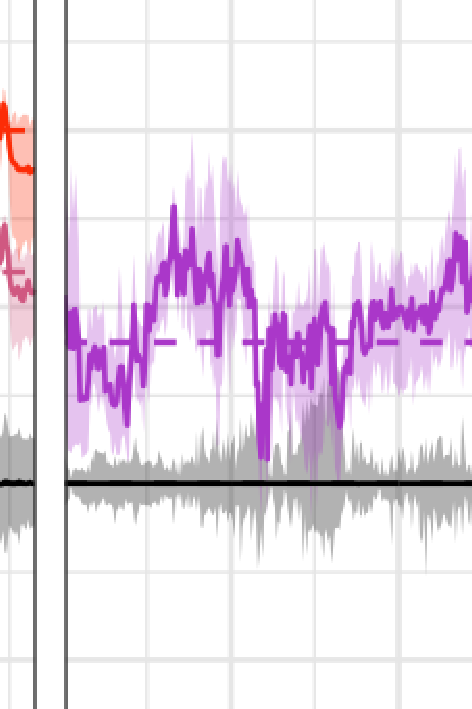
\includegraphics{/Users/aileneettinger/git/radcliffe/Analyses/figures/WarmingEffects_TimeSeries_SoilTemp1Mean_Deviation_NoPrecip.png}
 \caption{\textbf{Deviations in daily observed warming from mean control soil temperature for 12 study sites,} excluding data from plots that manipulated precipitation. We show soil, rather than above-ground, temperature, as this was the most frequently recorded temperature variable in the MC3E database. Solid lines show observed difference between warming treatment (colors) and control (black) plots, averaged across replicates and years; shading shows 95\% confidence intervals. Dashed lines represent target warming levels. (Note that the following studies had no explicit target temperature: exp06, exp11, exp12; for these studies, we used their reported level of warming.) Two sites not shown here did not monitor soil temperature. Experimental sites are ordered by low to high mean annual soil temperature (shown in the upper right corner of each panel). The heating type is listed in parentheses next to the site number (IR= infrared, soil= soil cables, air= forced air).} %The number of temperature treatment levels vary from one (e.g. exp08, exp11) to nine (exp07 and exp10, which used an unreplicated regression design). Daily temperature values were obtained by averaging across years for each day of the year in each temperature treatment in each study. 
 \label{fig:effwarm}
 \end{figure}

%%%%%%%%%%%%%%%%%%%%%%%%%%%%%%%%%%%%%%%%
\end{document}
%%%%%%%%%%%%%%%%%%%%%%%%%%%%%%%%%%%%%%%%
